%!TEX root = thesis.tex
\section{Multilayer Perceptron}\label{ch:Content2:sec:Section2}

\Glspl{MLP} are neural nets whichs neurons are structured in layers.
Each layer is fully connected with the next layer, but there are no other
connections between neurons.

\begin{figure}[ht]
    \centering
    %!TEX root = thesis.tex
\section{Multilayer Perceptron}\label{ch:Content2:sec:Section2}

\Glspl{MLP} are neural nets whichs neurons are structured in layers.
Each layer is fully connected with the next layer, but there are no other
connections between neurons.

\begin{figure}[ht]
    \centering
    %!TEX root = thesis.tex
\section{Multilayer Perceptron}\label{ch:Content2:sec:Section2}

\Glspl{MLP} are neural nets whichs neurons are structured in layers.
Each layer is fully connected with the next layer, but there are no other
connections between neurons.

\begin{figure}[ht]
    \centering
    %!TEX root = thesis.tex
\section{Multilayer Perceptron}\label{ch:Content2:sec:Section2}

\Glspl{MLP} are neural nets whichs neurons are structured in layers.
Each layer is fully connected with the next layer, but there are no other
connections between neurons.

\begin{figure}[ht]
    \centering
    \input{figures/feedforward.tex}
    \caption{Feedforward artificial neural network}
    \label{fig:feedforward}
\end{figure}

The red neurons in \cref{fig:feedforward} are input neurons, the green ones are
hidden neurons and the blue one is an output node. The gray neurons are bias neurons.
Bias neurons have a fixed output of $1$.

Usually, you have as many output neurons as you have classes. So in the case of
symbol recognition that would be about $\si{1076}$ neurons.

The number of input neurons is equal to the number of features.

Two neighboring layers of neurons are fully connected and have weights between
two layers. This means you can store those weights in form of matrices.
Assuming you have $n$ neurons in layer $i$ and $m$ neurons in layer $i + 1$,
you would have a matrix

\[W_{i} = \begin{pmatrix}
    w_{1,1} & w_{1,2} & \dots & w_{1,m}\\
    w_{2,1} & w_{2,2} & \dots & w_{2,m}\\
    w_{3,1} & w_{3,2} & \dots & w_{3,m}\\
    \vdots  &         & \ddots& \vdots \\
    w_{n,1} & w_{n,2} & \dots & w_{n,m}
\end{pmatrix}\]

This means you can easily get the input for layer $i+1$. As the input neurons
output is $x \in \mdr^{1 \times n}$ you can simply multiply $x \cdot W_1$
to get the output $x \cdot W_1 := \net_j \in \mdr^{1 \times m}$.

After that, you can apply the activation function $\varphi$ to $_i$.
As I assume that the activation function will be the same foreach node in the
same layer $l$, I will simply write $\varphi_l(o)$. This means that $\varphi_l$ is applied
componentwise to each $o_i$ with $i \in 1, \dots, m$.

So the output vector $o$ of a 3-layer (input, hidden, output) neural net can be
computed by

\[o = \varphi_2(\varphi_1(x \cdot W_{1,2}) \cdot W_{2,3})\]

The output of a general \gls{MLP} can be computed by

\begin{align*}
    \Phi(x, 1) &:= \varphi_{1}(x \cdot W_{1,2})\\
    \Phi(x, n) &:= \varphi_{n-1} \big (\Phi(x, n-1) \cdot W_{n-1, n} \big)
\end{align*}

\subsection{Supervised Training with Backpropagation}
The backpropagation algorithm is a supervised algorithm for training an
\gls{MLP}. This means the trainigset $T$ consists of tuples $(x, t)$
where $x$ is input and $t_x$ is the desired output.

The backpropagation algorithm first makes a forward pass to get to know what
the current output $o_x$ would be for each $(x, t_x) \in T$.
To evaluate how good the current \gls{MLP} is, an error function can be defined:

\begin{align*}
    E: \mdr^{n_1 \times n_2} \times \mdr^{n_2 \times n_3} \times \dots \times \mdr^{n_{m-1, m}} \rightarrow \mdr_{\geq 0}\\
    E_T(W) = \frac{1}{2} \sum_{(x, t_x) \in T} \sum_{k \in out} \left (t_{x}^{(k)} - o_{x}^{(k)} \right )^2
\end{align*}

where $n_i$ is the numer of neurons in the $i$-th layer and $m$ is the number
of layers and $out$ is the set of all output neurons.

This function is isomorphic to 

\[E: \mdr^{\sum_{i=2}^m n_{i-1} \cdot n_{i}} \rightarrow \mdr_{\geq 0}\]

This error should be minimized. As the error is the sum of non-negative values,
we will get a lower error by minimizing the error for a single training example.
However, note that those minimizations are not independant. This means, we could
get trapped in a local minimum.

The idea is to \enquote{go} into the direction in which the error $E$ decreases
most. This is the gradient and the process is thus called \textit{gradient descent}.

At this point we need to decide how far we want to go. If we make too big steps
in the direction of the gradient, we might overshoot. If we make too small steps,
the algorithm will take too long to get to the minimum. As reducing the error
is basically learning the number is called learning rate $\eta \in \mdr_{> 0}$.

So the algorithm is

\begin{algorithm}[h]
    \begin{algorithmic}
        \Function{backpropagate}{$T$, $W$}
            \While{True}
                \ForAll{$(x, t_x) \in T$}
                    \ForAll{node $i$}
                        \ForAll{nodes $j$ following $i$}
                            \State $\displaystyle w_{ij} \gets w_{ij} - \eta \frac{\partial E_{\Set{x}}}{\partial w_{ij}} (W)$
                        \EndFor
                    \EndFor
                \EndFor
            \EndWhile
        \EndFunction
    \end{algorithmic}
\caption{Backpropagate}
\label{alg:backpropagate}
\end{algorithm}

Computing the partial derivatives $\frac{\partial E_{\Set{x}}}{\partial w_{ij}}$
is not a trivial task. To do that, we have to take a closer look at the
error function:

Let $n$ be the number of layers of the \gls{MLP}.

\begin{align}
    \frac{\partial E_{\Set{x}}}{\partial w_{ij}}
    &= \frac{\partial}{\partial w_{ij}} \frac{1}{2} \sum_{(x, t_x) \in T} \sum_{k \in out} \left (t_{x}^{(k)} - o_{x}^{(k)} \right )^2\\
    &= \frac{1}{2} \sum_{(x, t_x) \in T} \sum_{k \in out} \frac{\partial}{\partial w_{ij}} \left (t_{x}^{(k)} - o_{x}^{(k)} \right )^2\\
    &= \frac{1}{2} \sum_{(x, t_x) \in T} \sum_{k \in out} 2 \left (t_{x}^{(k)} - o_{x}^{(k)} \right ) \cdot \frac{\partial}{\partial w_{ij}} \left (t_{x}^{(k)} - o_{x}^{(k)} \right )\\
    &= - \sum_{(x, t_x) \in T} \sum_{k \in out} \left (t_{x}^{(k)} - o_{x}^{(k)} \right ) \cdot \frac{\partial}{\partial w_{ij}} \left (\varphi_{n-1}(\Phi(x, n-1) \cdot W_{n-1,n})^{(k)} \right)
\end{align}

At this point, it doesn't get simpler except if you know where $w_{ij}$ is.
If $w_{ij}$ is for example a weight for an output node, you can apply the chain
rule\footnote{$(f(g))' = f'(g) \cdot g'$} once:

\begin{align}
    \frac{\partial E_{\Set{x}}}{\partial w_{ij}} &= - \sum_{(x, t_x) \in T} \sum_{k \in out} \left (t_{x}^{(k)} - o_{x}^{(k)} \right ) \cdot \left ( \frac{\partial}{\partial w_{ij}} \varphi_{n-1} \right )(\Phi(x, n-1) \cdot W_{n-1,n})^{(k)}\\
\end{align}
    \caption{Feedforward artificial neural network}
    \label{fig:feedforward}
\end{figure}

The red neurons in \cref{fig:feedforward} are input neurons, the green ones are
hidden neurons and the blue one is an output node. The gray neurons are bias neurons.
Bias neurons have a fixed output of $1$.

Usually, you have as many output neurons as you have classes. So in the case of
symbol recognition that would be about $\si{1076}$ neurons.

The number of input neurons is equal to the number of features.

Two neighboring layers of neurons are fully connected and have weights between
two layers. This means you can store those weights in form of matrices.
Assuming you have $n$ neurons in layer $i$ and $m$ neurons in layer $i + 1$,
you would have a matrix

\[W_{i} = \begin{pmatrix}
    w_{1,1} & w_{1,2} & \dots & w_{1,m}\\
    w_{2,1} & w_{2,2} & \dots & w_{2,m}\\
    w_{3,1} & w_{3,2} & \dots & w_{3,m}\\
    \vdots  &         & \ddots& \vdots \\
    w_{n,1} & w_{n,2} & \dots & w_{n,m}
\end{pmatrix}\]

This means you can easily get the input for layer $i+1$. As the input neurons
output is $x \in \mdr^{1 \times n}$ you can simply multiply $x \cdot W_1$
to get the output $x \cdot W_1 := \net_j \in \mdr^{1 \times m}$.

After that, you can apply the activation function $\varphi$ to $_i$.
As I assume that the activation function will be the same foreach node in the
same layer $l$, I will simply write $\varphi_l(o)$. This means that $\varphi_l$ is applied
componentwise to each $o_i$ with $i \in 1, \dots, m$.

So the output vector $o$ of a 3-layer (input, hidden, output) neural net can be
computed by

\[o = \varphi_2(\varphi_1(x \cdot W_{1,2}) \cdot W_{2,3})\]

The output of a general \gls{MLP} can be computed by

\begin{align*}
    \Phi(x, 1) &:= \varphi_{1}(x \cdot W_{1,2})\\
    \Phi(x, n) &:= \varphi_{n-1} \big (\Phi(x, n-1) \cdot W_{n-1, n} \big)
\end{align*}

\subsection{Supervised Training with Backpropagation}
The backpropagation algorithm is a supervised algorithm for training an
\gls{MLP}. This means the trainigset $T$ consists of tuples $(x, t)$
where $x$ is input and $t_x$ is the desired output.

The backpropagation algorithm first makes a forward pass to get to know what
the current output $o_x$ would be for each $(x, t_x) \in T$.
To evaluate how good the current \gls{MLP} is, an error function can be defined:

\begin{align*}
    E: \mdr^{n_1 \times n_2} \times \mdr^{n_2 \times n_3} \times \dots \times \mdr^{n_{m-1, m}} \rightarrow \mdr_{\geq 0}\\
    E_T(W) = \frac{1}{2} \sum_{(x, t_x) \in T} \sum_{k \in out} \left (t_{x}^{(k)} - o_{x}^{(k)} \right )^2
\end{align*}

where $n_i$ is the numer of neurons in the $i$-th layer and $m$ is the number
of layers and $out$ is the set of all output neurons.

This function is isomorphic to 

\[E: \mdr^{\sum_{i=2}^m n_{i-1} \cdot n_{i}} \rightarrow \mdr_{\geq 0}\]

This error should be minimized. As the error is the sum of non-negative values,
we will get a lower error by minimizing the error for a single training example.
However, note that those minimizations are not independant. This means, we could
get trapped in a local minimum.

The idea is to \enquote{go} into the direction in which the error $E$ decreases
most. This is the gradient and the process is thus called \textit{gradient descent}.

At this point we need to decide how far we want to go. If we make too big steps
in the direction of the gradient, we might overshoot. If we make too small steps,
the algorithm will take too long to get to the minimum. As reducing the error
is basically learning the number is called learning rate $\eta \in \mdr_{> 0}$.

So the algorithm is

\begin{algorithm}[h]
    \begin{algorithmic}
        \Function{backpropagate}{$T$, $W$}
            \While{True}
                \ForAll{$(x, t_x) \in T$}
                    \ForAll{node $i$}
                        \ForAll{nodes $j$ following $i$}
                            \State $\displaystyle w_{ij} \gets w_{ij} - \eta \frac{\partial E_{\Set{x}}}{\partial w_{ij}} (W)$
                        \EndFor
                    \EndFor
                \EndFor
            \EndWhile
        \EndFunction
    \end{algorithmic}
\caption{Backpropagate}
\label{alg:backpropagate}
\end{algorithm}

Computing the partial derivatives $\frac{\partial E_{\Set{x}}}{\partial w_{ij}}$
is not a trivial task. To do that, we have to take a closer look at the
error function:

Let $n$ be the number of layers of the \gls{MLP}.

\begin{align}
    \frac{\partial E_{\Set{x}}}{\partial w_{ij}}
    &= \frac{\partial}{\partial w_{ij}} \frac{1}{2} \sum_{(x, t_x) \in T} \sum_{k \in out} \left (t_{x}^{(k)} - o_{x}^{(k)} \right )^2\\
    &= \frac{1}{2} \sum_{(x, t_x) \in T} \sum_{k \in out} \frac{\partial}{\partial w_{ij}} \left (t_{x}^{(k)} - o_{x}^{(k)} \right )^2\\
    &= \frac{1}{2} \sum_{(x, t_x) \in T} \sum_{k \in out} 2 \left (t_{x}^{(k)} - o_{x}^{(k)} \right ) \cdot \frac{\partial}{\partial w_{ij}} \left (t_{x}^{(k)} - o_{x}^{(k)} \right )\\
    &= - \sum_{(x, t_x) \in T} \sum_{k \in out} \left (t_{x}^{(k)} - o_{x}^{(k)} \right ) \cdot \frac{\partial}{\partial w_{ij}} \left (\varphi_{n-1}(\Phi(x, n-1) \cdot W_{n-1,n})^{(k)} \right)
\end{align}

At this point, it doesn't get simpler except if you know where $w_{ij}$ is.
If $w_{ij}$ is for example a weight for an output node, you can apply the chain
rule\footnote{$(f(g))' = f'(g) \cdot g'$} once:

\begin{align}
    \frac{\partial E_{\Set{x}}}{\partial w_{ij}} &= - \sum_{(x, t_x) \in T} \sum_{k \in out} \left (t_{x}^{(k)} - o_{x}^{(k)} \right ) \cdot \left ( \frac{\partial}{\partial w_{ij}} \varphi_{n-1} \right )(\Phi(x, n-1) \cdot W_{n-1,n})^{(k)}\\
\end{align}
    \caption{Feedforward artificial neural network}
    \label{fig:feedforward}
\end{figure}

The red neurons in \cref{fig:feedforward} are input neurons, the green ones are
hidden neurons and the blue one is an output node. The gray neurons are bias neurons.
Bias neurons have a fixed output of $1$.

Usually, you have as many output neurons as you have classes. So in the case of
symbol recognition that would be about $\si{1076}$ neurons.

The number of input neurons is equal to the number of features.

Two neighboring layers of neurons are fully connected and have weights between
two layers. This means you can store those weights in form of matrices.
Assuming you have $n$ neurons in layer $i$ and $m$ neurons in layer $i + 1$,
you would have a matrix

\[W_{i} = \begin{pmatrix}
    w_{1,1} & w_{1,2} & \dots & w_{1,m}\\
    w_{2,1} & w_{2,2} & \dots & w_{2,m}\\
    w_{3,1} & w_{3,2} & \dots & w_{3,m}\\
    \vdots  &         & \ddots& \vdots \\
    w_{n,1} & w_{n,2} & \dots & w_{n,m}
\end{pmatrix}\]

This means you can easily get the input for layer $i+1$. As the input neurons
output is $x \in \mdr^{1 \times n}$ you can simply multiply $x \cdot W_1$
to get the output $x \cdot W_1 := \net_j \in \mdr^{1 \times m}$.

After that, you can apply the activation function $\varphi$ to $_i$.
As I assume that the activation function will be the same foreach node in the
same layer $l$, I will simply write $\varphi_l(o)$. This means that $\varphi_l$ is applied
componentwise to each $o_i$ with $i \in 1, \dots, m$.

So the output vector $o$ of a 3-layer (input, hidden, output) neural net can be
computed by

\[o = \varphi_2(\varphi_1(x \cdot W_{1,2}) \cdot W_{2,3})\]

The output of a general \gls{MLP} can be computed by

\begin{align*}
    \Phi(x, 1) &:= \varphi_{1}(x \cdot W_{1,2})\\
    \Phi(x, n) &:= \varphi_{n-1} \big (\Phi(x, n-1) \cdot W_{n-1, n} \big)
\end{align*}

\subsection{Supervised Training with Backpropagation}
The backpropagation algorithm is a supervised algorithm for training an
\gls{MLP}. This means the trainigset $T$ consists of tuples $(x, t)$
where $x$ is input and $t_x$ is the desired output.

The backpropagation algorithm first makes a forward pass to get to know what
the current output $o_x$ would be for each $(x, t_x) \in T$.
To evaluate how good the current \gls{MLP} is, an error function can be defined:

\begin{align*}
    E: \mdr^{n_1 \times n_2} \times \mdr^{n_2 \times n_3} \times \dots \times \mdr^{n_{m-1, m}} \rightarrow \mdr_{\geq 0}\\
    E_T(W) = \frac{1}{2} \sum_{(x, t_x) \in T} \sum_{k \in out} \left (t_{x}^{(k)} - o_{x}^{(k)} \right )^2
\end{align*}

where $n_i$ is the numer of neurons in the $i$-th layer and $m$ is the number
of layers and $out$ is the set of all output neurons.

This function is isomorphic to 

\[E: \mdr^{\sum_{i=2}^m n_{i-1} \cdot n_{i}} \rightarrow \mdr_{\geq 0}\]

This error should be minimized. As the error is the sum of non-negative values,
we will get a lower error by minimizing the error for a single training example.
However, note that those minimizations are not independant. This means, we could
get trapped in a local minimum.

The idea is to \enquote{go} into the direction in which the error $E$ decreases
most. This is the gradient and the process is thus called \textit{gradient descent}.

At this point we need to decide how far we want to go. If we make too big steps
in the direction of the gradient, we might overshoot. If we make too small steps,
the algorithm will take too long to get to the minimum. As reducing the error
is basically learning the number is called learning rate $\eta \in \mdr_{> 0}$.

So the algorithm is

\begin{algorithm}[h]
    \begin{algorithmic}
        \Function{backpropagate}{$T$, $W$}
            \While{True}
                \ForAll{$(x, t_x) \in T$}
                    \ForAll{node $i$}
                        \ForAll{nodes $j$ following $i$}
                            \State $\displaystyle w_{ij} \gets w_{ij} - \eta \frac{\partial E_{\Set{x}}}{\partial w_{ij}} (W)$
                        \EndFor
                    \EndFor
                \EndFor
            \EndWhile
        \EndFunction
    \end{algorithmic}
\caption{Backpropagate}
\label{alg:backpropagate}
\end{algorithm}

Computing the partial derivatives $\frac{\partial E_{\Set{x}}}{\partial w_{ij}}$
is not a trivial task. To do that, we have to take a closer look at the
error function:

Let $n$ be the number of layers of the \gls{MLP}.

\begin{align}
    \frac{\partial E_{\Set{x}}}{\partial w_{ij}}
    &= \frac{\partial}{\partial w_{ij}} \frac{1}{2} \sum_{(x, t_x) \in T} \sum_{k \in out} \left (t_{x}^{(k)} - o_{x}^{(k)} \right )^2\\
    &= \frac{1}{2} \sum_{(x, t_x) \in T} \sum_{k \in out} \frac{\partial}{\partial w_{ij}} \left (t_{x}^{(k)} - o_{x}^{(k)} \right )^2\\
    &= \frac{1}{2} \sum_{(x, t_x) \in T} \sum_{k \in out} 2 \left (t_{x}^{(k)} - o_{x}^{(k)} \right ) \cdot \frac{\partial}{\partial w_{ij}} \left (t_{x}^{(k)} - o_{x}^{(k)} \right )\\
    &= - \sum_{(x, t_x) \in T} \sum_{k \in out} \left (t_{x}^{(k)} - o_{x}^{(k)} \right ) \cdot \frac{\partial}{\partial w_{ij}} \left (\varphi_{n-1}(\Phi(x, n-1) \cdot W_{n-1,n})^{(k)} \right)
\end{align}

At this point, it doesn't get simpler except if you know where $w_{ij}$ is.
If $w_{ij}$ is for example a weight for an output node, you can apply the chain
rule\footnote{$(f(g))' = f'(g) \cdot g'$} once:

\begin{align}
    \frac{\partial E_{\Set{x}}}{\partial w_{ij}} &= - \sum_{(x, t_x) \in T} \sum_{k \in out} \left (t_{x}^{(k)} - o_{x}^{(k)} \right ) \cdot \left ( \frac{\partial}{\partial w_{ij}} \varphi_{n-1} \right )(\Phi(x, n-1) \cdot W_{n-1,n})^{(k)}\\
\end{align}
    \caption{Feedforward artificial neural network}
    \label{fig:feedforward}
\end{figure}

The red neurons in \cref{fig:feedforward} are input neurons, the green ones are
hidden neurons and the blue one is an output node. The gray neurons are bias neurons.
Bias neurons have a fixed output of $1$.

Usually, you have as many output neurons as you have classes. So in the case of
symbol recognition that would be about $\si{1076}$ neurons.

The number of input neurons is equal to the number of features.

\section{Notation}
Let $n_i$ be the number of neurons in the $i$-th layer and $\layernumber$ be the
number of layers of the \gls{MLP}.

Two neighboring layers of neurons are fully connected and have weights between
two layers. This means you can store those weights in form of matrices.
So the weights between layer $i$ and layer $i+1$ are

\[W_i = \begin{pmatrix}
    w_{1,1} & w_{1,2} & \dots & w_{1,n_{i+1}}\\
    w_{2,1} & w_{2,2} & \dots & w_{2,n_{i+1}}\\
    w_{3,1} & w_{3,2} & \dots & w_{3,n_{i+1}}\\
    \vdots  &         & \ddots& \vdots \\
    w_{n_{i},1} & w_{n_{i},2} & \dots & w_{n_{i},n_{i+1}}
\end{pmatrix}\]

Let $w_{ij}^{(k)}$ be the value $w_{ij}$ in $W_k$. So it is the weight of the
between neuron $i$ in layer $k$ and neuron $j$ in layer $k+1$.

So $W_i \in \mdr^{n_i \times n_{i+1}}$ is the matrix denoting the weights between layer
$i$ and layer $i+1$.

The unweighted output vector of layer $i$ is denoted by $x_i \in \mdr^{1 \times n_i}$;
the weighted output vector by $\net_i \in \mdr^{1 \times n_i}$. Instead of $x_1$ I
will write $x$.
The output of the \gls{MLP} for the input $x$ is denoted by $o_x:= x_n$.

In principle each neuron might have a different activation function, but in
practice each neuron in one layer has the same activation function. However,
activation functions might differ from layer to layer. This is the reason why
I denote the activation function of layer $i$ by $\varphi_i$. Although $\varphi_i$
is defined for single neurons, I will in the following apply it to vectors. In
its meant to be applied pointwise.

The activation function is a function 

\[\varphi_i: \mdr \rightarrow \mdr \]

but because of the short-notation it can be applied pointwise to all neurons
of layer $i$ it is also a function

\[\varphi_i: \mdr^{n_{i}} \rightarrow \mdr^{n_{i}}\]

\section{Evaluation}
Let $x_1 \in \mdr^{1 \times n_1}$ be an unweighted output of layer $1$. So it's
simply the input of our neural net with $n_1$ features.

Given $x_1$ one can easily compute the weighted input for layer $2$:

\[
\begin{array}{@{}c@{\;}c@{\;}c@{\;}c@{\;}c@{}}
x_1 & \cdot & W_{1} & = & \net_1 \\
\vin && \vin && \vin \\
\mathbb{R}^{1\times n_1} && \mathbb{R}^{n_1\times n_2} && \mathbb{R}^{1\times n_2}
\end{array}
\]

After that, you can apply the activation function $\varphi_{i+1}$ pointwise
to $\net_i$.\todo{Is that really called "pointwise" application?}

So the output vector $x_3$ of a 3-layer (input, hidden, output) neural net can be
computed by

\[x_3 = \varphi_3(\varphi_2(x_1 \cdot W_{1}) \cdot W_{2})\]

The output of a general \gls{MLP} can be computed by

\begin{align*}
    \Phi(x, n) &: \mdr^{n_1} \rightarrow \mdr^{n_n}\\
    \Phi(x_1, 2) &:= \varphi_{2}(x_1 \cdot W_{1})\\
    \Phi(x, n) &:= \varphi_{n} \left (\Phi(x, n-1) \cdot W_{n-1} \right)\\
    \Phi(x, n)^{(p)} &= \varphi_n \left ( \sum_{i=1}^{n_{n-1}} \Phi(x, n-1)^{(i)} \cdot w_{ip}^{(n-1)} \right )
\end{align*}

It follows: $x_i(x_1) = \Phi(x_1, i)$.

\section{Supervised Training with Backpropagation}\label{sec:training}
The backpropagation algorithm is a supervised algorithm for training
\glspl{MLP}. This means the trainigset $T$ consists of tuples $(x, t_x)$
where $x$ is input and $t_x$ is the desired output.

To evaluate how good the current \gls{MLP} is, an error function can be defined:

\begin{align*}
    E: \mdr^{n_1 \times n_2} \times \mdr^{n_2 \times n_3} \times \dots \times \mdr^{n_{\layernumber-1, \layernumber}} \rightarrow \mdr_{\geq 0}\\
    E_T(W) = \frac{1}{2} \sum_{(x, t_x) \in T} \sum_{p = 1}^{n_\layernumber} \left (t_{x}^{(p)} - o_{x}^{(p)} \right )^2
\end{align*}

This function is isomorphic to 

\[E: \mdr^{\sum_{i=2}^\layernumber n_{i-1} \cdot n_{i}} \rightarrow \mdr_{\geq 0}\]

This error should be minimized. As the error is the sum of non-negative values,
we will get a lower error by minimizing the error for a single training example.
However, note that those minimizations are not independant. This means, we could
get trapped in a local minimum.

The idea is to \enquote{go} into the direction in which the error $E$ decreases
most. This is the gradient and the process is thus called \textit{gradient descent}.

At this point we need to decide how far we want to go. If we make too big steps
in the direction of the gradient, we might overshoot. If we make too small steps,
the algorithm will take too long to get to the minimum. As reducing the error
is basically learning the number is called learning rate $\eta \in \mdr_{> 0}$.

So the algorithm is

\begin{algorithm}[h]
    \begin{algorithmic}
        \Function{backpropagate}{$T$, $W$}
            \While{True}
                \ForAll{$(x, t_x) \in T$}
                    \ForAll{node $i$}
                        \ForAll{nodes $j$ following $i$}
                            \State $\displaystyle w_{ijk} \gets w_{ijk} - \eta \frac{\partial E_{\Set{x}}}{\partial w_{ijk}} (W)$
                        \EndFor
                    \EndFor
                \EndFor
            \EndWhile
        \EndFunction
    \end{algorithmic}
\caption{Backpropagate}
\label{alg:backpropagate}
\end{algorithm}

Computing the partial derivatives $\frac{\partial E_{\Set{x}}}{\partial w_{ijk}}$
is not a trivial task. To do that, we have to take a closer look at the
error function:

\begin{align}
    E_x(W) &= \frac{1}{2} \sum_{p=1}^{n_\layernumber} \left ( t_x^{(p)} -o_x^{(p)} \right )^2\\
    o_x^{(p)} &= \Phi(x, \layernumber)^{(p)} \\
              &= \varphi_{\layernumber} \big (\Phi(x, \layernumber-1) \cdot W_{\layernumber-1} \big)^{(p)}\\
              &= \varphi_{\layernumber} \big (
                  \underbrace{
                      \sum_{i=1}^{n_{\layernumber-1}} \Phi(x, \layernumber-1)^{(i)} \cdot w_{ip}^{(\layernumber-1)}
                  }_{\net_{\layernumber-1}^{(p)}} \big)\\
    \frac{\partial E_x}{\partial w_{ij}^{(k)}} &= \frac{\partial E_x}{\partial \net_k^{(j)}} \frac{\partial \net_k^{(j)}}{\partial w_{ij}^{(k)}}\\
    &= \frac{\partial E_x}{\partial \net_k^{(j)}} \frac{\sum_{i=1}^{n_{k}} \Phi(x, k)^{(i)} \cdot w_{ij}^{(k)}}{\partial w_{ij}^{(k)}}\\
    &= \frac{\partial E_x}{\partial \net_k^{(j)}} \Phi(x, k)^{(i)}
\end{align}

Suppose $k = \layernumber - 1$ (weights to the output layer). Then:

\begin{align}
    \frac{\partial E_x}{\partial w_{ij}^{(\layernumber-1)}} &= \frac{\partial E_x}{\partial \net_{\layernumber-1}^{(j)}} \Phi(x, \layernumber-1)^{(i)}\\
    &= \frac{\frac{1}{2} \sum_{p=1}^{n_\layernumber} \left ( t_x^{(p)} -o_x^{(p)} \right )^2}{\partial \net_{\layernumber-1}^{(j)}} \Phi(x, \layernumber-1)^{(i)}\\
    &= \frac{\frac{1}{2} \sum_{p=1}^{n_\layernumber} \left ( t_x^{(p)} -\varphi_{\layernumber}(\net_{\layernumber-1})^{(p)} \right )^2}{\partial \net_{\layernumber-1}^{(j)}} \Phi(x, \layernumber-1)^{(i)}\\ % I can put this to the top
    &= \left (
            (t_x^{(j)} - \varphi_{\layernumber}(\net_{\layernumber-1}^{(j)})) \cdot (- \varphi_{\layernumber}'(\net_{\layernumber-1}^{(j)}))
       \right ) \Phi(x, \layernumber-1)^{(i)}
\end{align}

%If you further assume that $\varphi_{}$

Suppose $k = \layernumber - 2$ (last hidden layer). Then:

\begin{align}
    \frac{\partial E_x}{\partial w_{ij}^{(\layernumber-2)}} &= \frac{\frac{1}{2} \sum_{p=1}^{n_\layernumber} \left ( t_x^{(p)} -\varphi_{\layernumber}(\net_{\layernumber-1})^{(p)} \right )^2}{\partial \net_{\layernumber-2}^{(j)}} \Phi(x, \layernumber-2)^{(i)}\\
    &= \frac{\frac{1}{2} \sum_{p=1}^{n_\layernumber} \left ( t_x^{(p)} -\varphi_{\layernumber}(\sum_{i=1}^{n_{\layernumber-1}} (
        \varphi_{\layernumber-1} \big (\varphi_{\layernumber-2}(\net_{\layernumber-2}^{(j)}) \big)
    )^{(i)} \cdot w_{ip}^{(\layernumber-1)})^{(p)} \right )^2}{\partial \net_{\layernumber-2}^{(j)}} \Phi(x, \layernumber-2)^{(i)}\\
\end{align}

\section{Parameters}
\begin{itemize}
    \item Number of hidden layers
    \item Number of neurons per hidden layer
    \item \Glspl{epoch}
    \item Momentum
    \item Weight decay
    \item \Gls{learning rate}
    \item \Gls{learning rate decay}
\end{itemize}

%!TEX root = thesis.tex
\section{Activation functions}
\begin{figure}[ht]
    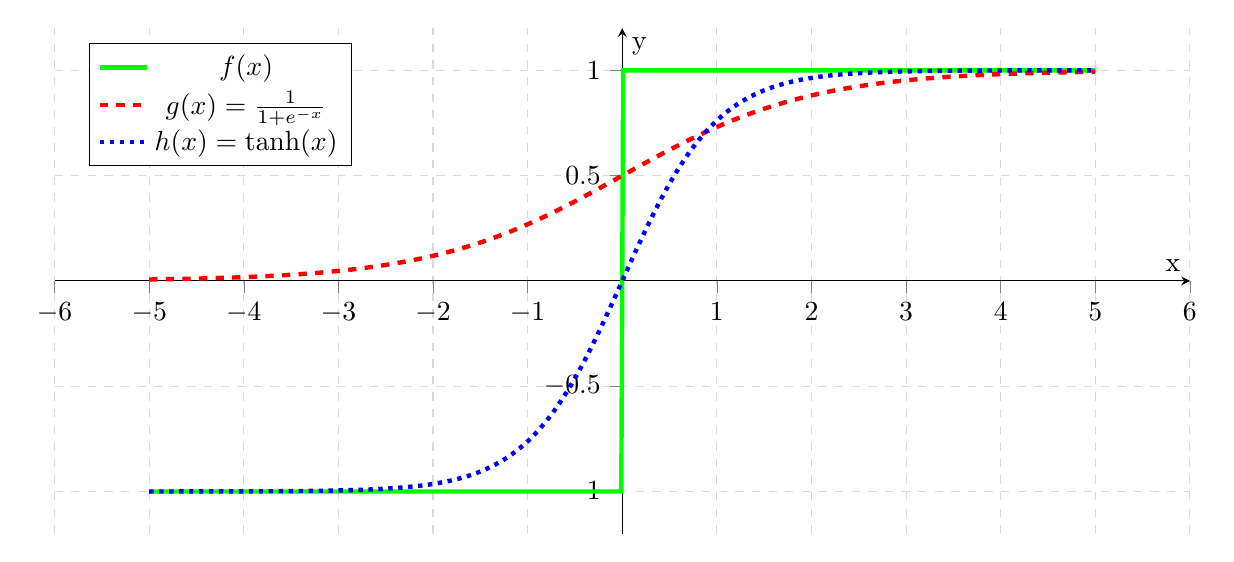
\begin{tikzpicture}[scale=1.0]
        \begin{axis}[
            legend pos=north west,
            axis x line=middle,
            axis y line=middle,
            grid = major,
            width=16cm,
            height=8cm,
            grid style={dashed, gray!30},
            xmin=-5,     % start the diagram at this x-coordinate
            xmax= 5,    % end   the diagram at this x-coordinate
            ymin=-1,     % start the diagram at this y-coordinate
            ymax= 1,   % end   the diagram at this y-coordinate
            %axis background/.style={fill=white},
            xlabel=x,
            ylabel=y,
            tick align=outside,
            enlargelimits=true]
          \addplot[domain=-5:5, green, ultra thick,samples=500] {x < 0 ? -1 : 1};
          \addplot[domain=-5:5, red, ultra thick,samples=500, dashed] {1/(1+exp(-x))};
          \addplot[domain=-5:5, blue, ultra thick,samples=500, dotted] {tanh(x)};
          \addlegendentry{$f(x)$}
          \addlegendentry{$g(x)=\frac{1}{1+e^{-x}}$}
          \addlegendentry{$h(x)=\tanh(x)$}
        \end{axis} 
    \end{tikzpicture}
    \caption{A variation of the sign function $f$ with $f(0) = -1$, the sigmoid function $g$ and the hyperbolic tangend $h$.}
    \label{fig:logistic-function}
\end{figure}

\subsection{Unit step function}\label{f:unitstep}
Not so good, because it's not differentiable. Therefore, the backpropagation
algorithm cannot be used.

\subsection{Sigmoid function}\label{f:sigmoid}
Is great because it is infinitely often differentiable.


\subsection{Hyperbolic tangent}\label{f:tanh}
Also differentiable, but gradient descent converges faster (sometimes?)

\subsection{Softmax}\label{f:softmax}

\[\varphi(a_j) = \frac{e^{a_j}}{\sum_k e^{a_k}}\]

\section{Out of Vocabulary}
It might be desirable to have a possibility to reject drawings that were not
recognized. Such a rejection could be realized in two ways:

\begin{itemize}
    \item A threshold for the answer,
    \item a minimum delta between the highest rated answer and the second
          highest rated answer or
    \item explicitly training for \gls{OOV}.
\end{itemize}

\section{Time Delay Neural Networks}

Time Delay Neural Networks were successfully applied to symbol recognition task
in the past\cite{Guyon91,Manke01}.

TODO!